\documentclass[__main__.tex]{subfiles}

\begin{document}

\qtitle{16}
Метод касательных (Ньютона) для решения алгебраических уравнений.


Рассмотрим функцию $f \in C^2([a;b], \mathbb R)$, удовлетворяющая условиям:
\begin{enumerate}
	\item $f(a)<0$ и $f(b)>0$ (или наоборот)
	\item $f'>0$ на $[a;b]$ (или наоборот)
	\item $f''\geqslant 0$ на $[a;b]$
\end{enumerate}

$$
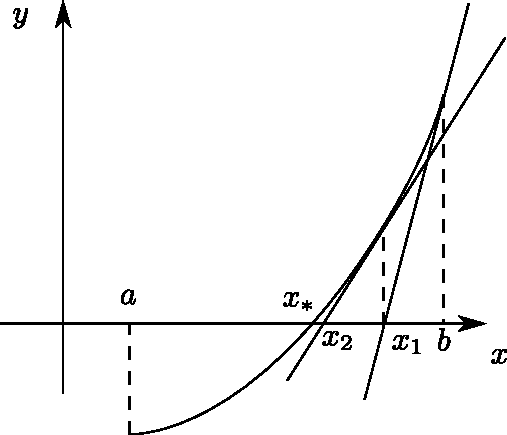
\includegraphics[scale=0.8]{img/16.pdf}
$$
На отрезке $[a;b]$ рассмотрим уравнение:
\begin{gather*}
\left\{
\begin{gathered}
f(x)=0 \hfill \\
x \in [a;b]
\end{gathered}	
\right.
\end{gather*}
где $x_* \in [a;b]$ --- решение уравнения (единственное).\\
Для численного решения уравнения используется метод ростой итерации $\operatorname{itr}(\varphi, x_0$, где $\varphi(x)=x-((f'(x))^{-1}\cdot f(x)$ для $x \in [a;b]$ и $x_0 \in (x_*; b)$ (или $x_0\in(a;x_0)$).\\

Рабочая формула этого метода имеет вид:
\begin{gather*}
x_k=x_{k-1}-((f'(x_{k-1}))^{-1}f(x_{k-1})), \qquad k\in \mathbb N
\end{gather*}
Из рабочей формулы следует:
\begin{gather*}
f(x_{k-1})+f'(x_{k-1})(x_k-x_{k-1})=0
\end{gather*}
То есть точка $x_k\in (a;b)$ является абсциссой точки пересечения касательной к кривой $y=f(x)$, проходящей через точку $(x_{k-1}; f(x_{k-1})$, с осью $OX$.\\

Такой метод простой итерации называют методом касательных или методом Ньютона.

Поскольку $\varphi(x)=x-((f'(x))^{-1}\cdot f(x)$ для $x \in (x_*, b]$, то 
\begin{gather*}
\varphi ' (x) = \frac{f''(x)f(x)}{(f'(x))^2} \longrightarrow 0 \mbox{ при } x \rightarrow x_*
\end{gather*}
Поэтому скорость сходимости метода квадратичная, если $x_0$ достаточно близко к $x_*$.
\end{document}